\section{Processing Input}

Initially, input to PyPltRedex is read from the file and stored as a string. To be able to apply reduction-relation, the string needs to be analyzed. There are two parts:

\begin{itemize}
\item
Lexical analysis that breaks up the string into individual tokens and decides which kind of token it is.
\item
Parsing - given a set of tokens, produce valid terms.
\end{itemize}


\subsection{Lexical Analysis}

Most commonly tokens are described using regular expressions. Below is description of token kinds supported by PyPltRedex.
\begin{itemize}
\item
	TODO maybe more visual regex display.
\end{itemize}

\subsection{Parsing}

Parsing takes individual lexemes and creates structured data out of them. In this case, terms are produced. Terms have the following grammar:

\begin{lstlisting}
term = term-sequence atom
term-sequence = (term ...) 
atom = integer 
	 | string
	 | (-|+)?[0-9]+\.[0-9]+
	 | #t
	 | #f
	 | identifier
\end{lstlisting}


\subsection{Implementation}
Class diagram for both \texttt{Tokenizer} and \texttt{Parser} can be seen in Figure \ref{class-diagram-lexer-parser}.

\begin{figure}[h]
	\centering
	\makebox[\textwidth][c] { 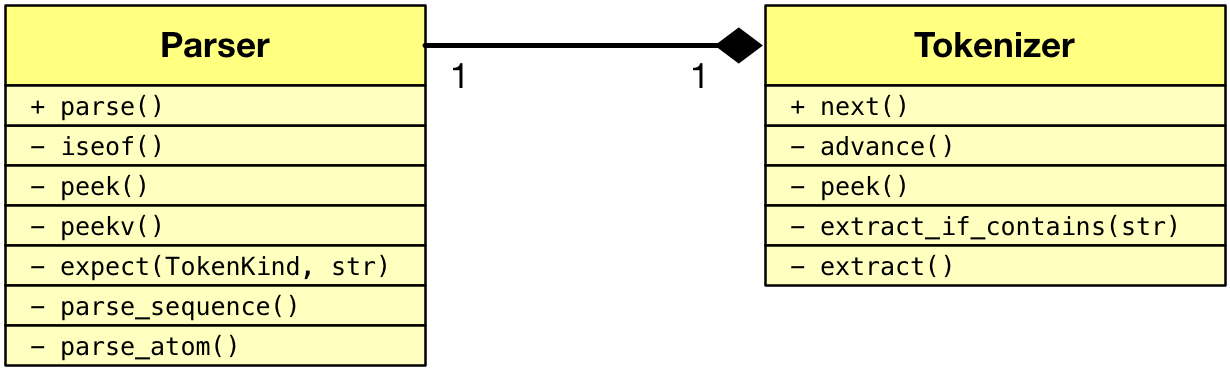
\includegraphics[scale=0.30]{class-diagram-lexer-parser.png} }
\caption{Class diagram for \texttt{Tokenizer} and \texttt{Parser}.}
\label{class-diagram-lexer-parser}
\end{figure}

Actual lexer implementation doesn't use regular expressions that were described above but implements their functionality using manually implemented state machine. The following functions are used to classify symbols:

\begin{lstlisting}
def is_whitespace(c):
    return c == ' ' or c == '\t' or c == '\n' or c == '\r'

def is_newline(c):
    return c == '\n'

def is_reserved(c): 
    return c in ['(', ')', '[', ']', '{', '}', '\"', '\'', '`', ';', '#', '|', '\\']

def is_digit(c):
    return c in ['0', '1', '2', '3', '4', '5', '6', '7', '8', '9']

def is_plusminus(c):
    return c in ['-', '+']

def is_delimeteter(c):
    return is_reserved(c) or c == '\0' or is_whitespace(c)

def is_leftparen(c):
	return c in ['(', '[', '{']

def is_rightparen(c):
	return c in [')', ']', '}']

\end{lstlisting}


\begin{itemize}
\item
\texttt{string} is the string that requires lexical analysis.

\item
\texttt{start} and \texttt{end} are indices indicating an interval within the \texttt{string}. The substring that ends with index \texttt{start} has already been analyzed. A substring between \texttt{start} and \texttt{end} is a potential token. Any substring after \texttt{end} requires analysis.

\item
\texttt{advance()} method increments \texttt{end} by one.

\item
\texttt{peek()} returns a character at index \texttt{end} of the \texttt{string}.
\texttt{extract\_if\_contains(substring)} extracts substring \texttt{s} beginning at \texttt{start} and ending at \texttt{start+len(substring)} and compares it against provided \texttt{substring}. If both strings are equal, \texttt{start} and \texttt{end} indices are set to \texttt{start+len(substring)} and True is returned. Otherwise, False is returned.

\item
\texttt{extract()} extracts the string between \texttt{start} and \texttt{end}, sets \texttt{start=end} and returns the extracted string.

\item
	\texttt{next()} returns the next token in the string. This method implements actual tokenization logic. All regular expressions are implemented directly instead of using RPython's regular expression library (for reasons why see below). State machine representing this method can be seen in Figure \ref{lexical-analysis-tokenize}.

\begin{figure}[th!]
	\centering
	\makebox[\textwidth][c] { 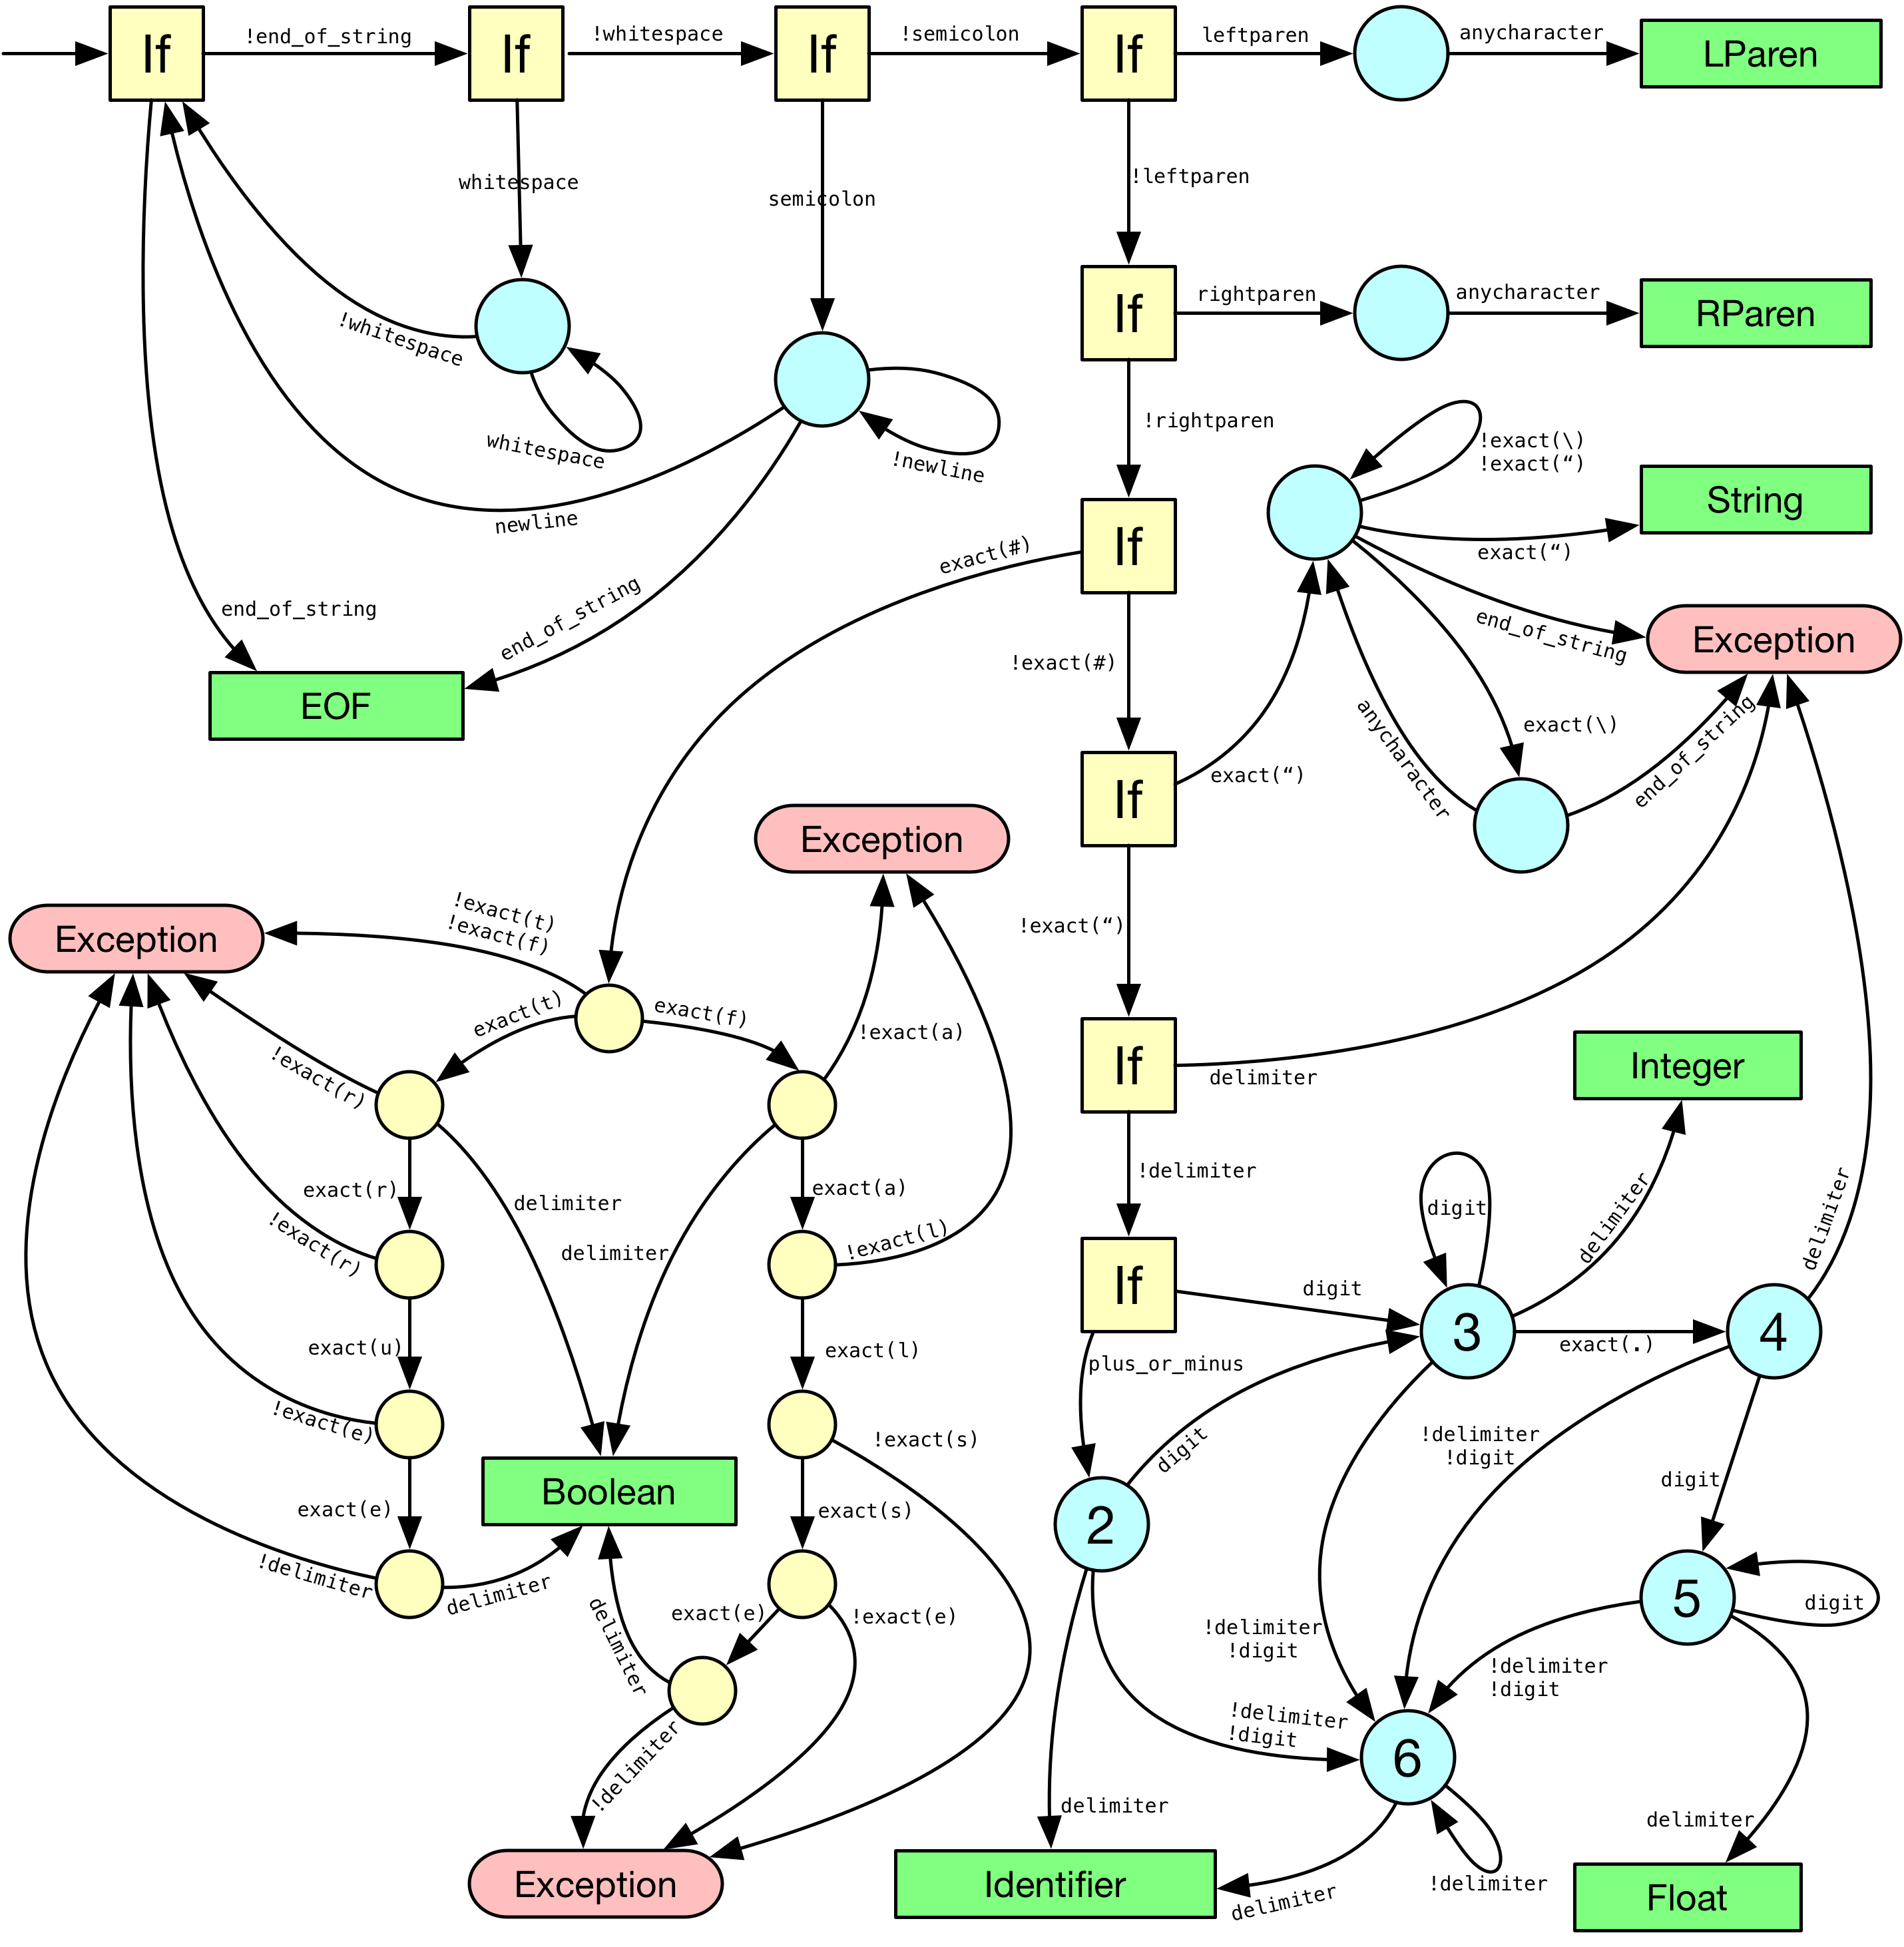
\includegraphics[scale=0.16]{lexical-analysis-tokenize.png} }
\caption{State machine for lexical analysis.}
\label{lexical-analysis-tokenize}
\end{figure}

Edges of the graph represent calls to \texttt{peek()} and ensuring the character satisfies a predicate an edge is labeled with. Taking a transition does not consume any characters. Predicates are described above.

The state machine has different node types with different character consumption strategies.
\begin{itemize}
\item states that return tokens annotated with their types, highlighted in green. After moving to this state no input is consumed.
\item states that raise Exceptions highlighted in red. After moving to this state no input is consumed.
\item \texttt{If} states are essentially \texttt{if} statements. They consume no characters.
\item Circled blue states actually consume characters. They also may have self-loops indicating consumption of one or more characters satisfying given predicate.
\item Circled yellow states are conceptually identical to blue states but are handled differently as explained below.
\end{itemize}

The state machine proceeds in the following manner

\begin{enumerate}
\item First ensure end of the string has not been reached, otherwise return (Eof)
\item Then, if current character whitespace, go to the state $s1$ that consumed all whitespace characters. Go back to the beginning and perform "end of the string" check.
\item After moving to state $if3$ and if current character is semicolon indicating beginning of comment, go to state $s2$ that consumes anything that is not a newline or end-of-the-string. Comment is then discarded and state machine transitions either to $if1$ or $eof$ returning (Eof).
\item Next two If statements detect closing and opening parantheses/braces/brackets and return (Lbrace) or (Rprace) accordingly.
\item If current character starts with pound sign indicating possible boolean, goto state $s3$. These yellow states do not consume input character by character but utilize \texttt{extract\_if\_contains} peek and consume multiple characters at once. This method is called in following manner:
\begin{itemize}
\item
if \texttt{extract\_if\_contains("\#t")} return (Boolean "\#t)
\item
if \texttt{extract\_if\_contains("\#f")} return (Boolean "\#f)
\item
if \texttt{extract\_if\_contains("\#true")} return (Boolean "\#t)
\item
if \texttt{extract\_if\_contains("\#false")} return (Boolean "\#f)
\end{itemize}

\item If current character is double quote, consume any character until closing double quote is found. Escape sequences are supported expecting a single character after backward slash. If end-of-string is encountered prematurely, Exception is raised. Otherwise, (String, \texttt{self.extract()}) is returned.

\item Finally, at this point a token can only be an integer, float, or identifier. This state machine is more complex.

\begin{itemize}
\item After arriving into state $1$, next character can either be (1) plus or minus thus moving to state 2;  (2) digit thus moving to state 3; (3) any other symbol that is not a delimeter this moving to state 6; and (4) delimiter thus moving to Exception state.
\item After arriving to state $2$ and consuming \texttt{+} or \texttt{-}, next character can either be (1) digit -> 3; (2) delimeter -> returning (Identifier, \texttt{extract()}) as \texttt{-} or \texttt{+} are valid identifiers in Racket; (3) Any other symbol that is not delimeter -> 6.
\item After arriving to state 3 and consuming a digit, next character can either be (1) a digit -> 3 (implemented as \texttt{while} loop); (2) delimeter thus returning (Integer, extract()); (3) fullstop symbol -> 4 indicating potential floating point number; (4) character that is neither a delimeter/number/nor fullstop -> 6.
\item After arriving to state 4 and consuming fullstop, next character can either be (1) delimeter -> raise Exception because fractional part of the float is missing; (2) digit -> 5; (3)neither a digit or delimeter -> 6.
\item After arriving to state 5 and consuming a digit, next character can either be (1) digit -> 5 (again, implemented as \texttt{while} loop); (2) delimeter -> return (Float, extract()) (3) neither a digit nor delimeter -> 6.
\item After arriving to state 6 and consuming some character, next character can either be (1) delimeter - return (Ident, extract()); (2) not delimeter -> 6.

\end{itemize}
This completes state machine description
\end{enumerate}

\end{itemize}

This completes description of the tokenizer. The parser is implemented as a very simple recursive descent parser. Below follows the description of its methods and their functionalities.

\begin{itemize}
\item
\texttt{iseof()} returns true if end of the string has been reached.

\item
\texttt{peek()} returns kind of the next token. 

\item
\texttt{peekv()} returns kind of the next token along with it's value.

\item 
\texttt{expect(expectedkind, tok=None)} throws Exception when \texttt{currenttoken} is not the one expected. In particular,
	\begin{itemize}
		\item
		If \texttt{expectedkind != nexttoken.kind} raise Exception.
		\item
		If \texttt{tok != None}, additionally check if \texttt{tok=nexttoken.value}. Raise Exception if it is not.
		\item
		Otherwise, call \texttt{tokenizer.next()} and assign it to \texttt{nexttoken} and return previous token. 
	\end{itemize}

\item 
	\texttt{parse\_sequence} implements parsing of \texttt{term-sequence} from the grammar above
	\begin{itemize}
		\item
		Let \texttt{seq} be an empty list.

		\item
		The first token is expected to be \texttt{LParen}.

		\item
		While \texttt{peek()} is not \texttt{RParen}, if \texttt{peek()} is \texttt{LParen}, call \texttt{term-sequence} and append its result to \texttt{seq}, otherwise call \texttt{parse\_atom} and append its result to seq.
	
		\item
		\texttt{expect(RParen)} 

		\item
		Return \texttt{Sequence(seq)}
	\end{itemize}

\item
\texttt{parse\_atom} implements parsing of \texttt{atom} from grammar.
	\begin{itemize}
	\item
		If \texttt{peek()} is Integer, return \texttt{Integer(expect(Integer))}
	\item
		If \texttt{peek()} is Float, return \texttt{Float(expect(Decimal))}
	\item

		If \texttt{peek()} is String, return \texttt{String(expect(String))}
	\item
		If \texttt{peek()} is Boolean, return \texttt{Boolean(expect(Boolean))}
	\item

		If \texttt{peek()} is Ident, then \texttt{peekv} to retrieve the value of the token. If value of token is \texttt{hole} return \texttt{Hole()}, otherwise Variable(self.expect(Ident)).
	\end{itemize}
	

\end{itemize}

\subsection{Implementation: Difficulties}
Initial lexical analysis implementation relied on regular expression library provided by RPython for identifying integers, floating point numbers and identifiers using regular expressions described in section TODO. While library works fine while running the lexer using \texttt{python2.7}, attempting to compile lexer code using \texttt{rpython} toolchain results in the following compilation error:

\begin{lstlisting}
[translation:ERROR] AttributeError: 'FrozenDesc' object has no attribute 'pycall'
Processing block:
 block@1149[_choice5_0...] is a <class 'rpython.flowspace.flowcontext.SpamBlock'> 
 in (rpython.rlib.parsing.regexparse:1495)RegexParser._charclass 
 containing the following operations: 
       v1 = simple_call((type set), v0) 
       v2 = simple_call((builtin_function range), (97), (123)) 
       v3 = newlist() 
       v4 = iter(v2) 
       v5 = hint(v3, v2, ({'maxlength': True})) 
\end{lstlisting}

Seems like RPython's \texttt{RegexParser} functionality has a bug. After attempting to investigate, I decided (TODO passive voice) to implement these regular expressions manually instead of relying on the library. This decision was made also because construction of those regular expressions was rather slow.

\subsection{Future Improvements}
TODO compare performance on big terms. 
float lexing is not faithful .3 and 1. are vaild floats
scientific notation 1e03 is not supported and parsed as identifer.

